\section{Modelagem no espaço das juntas}
Manipuladores subatuados diferem dos totalmente atuados pois são equipados com um número de atuadores que é sempre menor que o número de graus de liberdade (GDL). Portanto, nem todos os GDL podem ser controlados ativamente ao mesmo tempo \cite{Sbornian2004}. Por exemplo, com um manipulador planar de 3 juntas equipado com dois atuadores, ou seja, duas juntas ativas e
uma passiva, pode-se controlar ao mesmo tempo duas das juntas a qualquer instante, mas não todas. Para controlar todas as juntas de um manipulador subatuado, deve-se usar um controle sequencial. Este princípio foi provado pela primeira vez por {arai} usando  argumentos dinâmicos linearizados \cite{Joea2003}, e é a base para a modelagem no espaço das juntas e no espaço Cartesiano. A Tabela \ref{minhatab} apresenta os resultados \cite{Assenmacher1993,Silberschatz1991,Caromel1998}.

\begin{table}
\caption{Exemplo de uma Tabela}
\label{minhatab}

\center
\begin{tabular}{cccc}
  % after \\: \hline or \cline{col1-col2} \cline{col3-col4} ...
  \hline
	Parâmetro & Unidade & Valor da simulação & Valor experimental   \\
	\hline
  Comprimento, $\alpha$ & $m$ &  $8,23$  & $8,54$ \\
  Altura, $\beta$ & $m$     &  $29,1$ & $28,3$\\
	Velocidade, $v$ & $m/s$  &  $60,2$ & $67,3$\\
	\hline
\end{tabular}
\end{table}

Devido ao fato de que no máximo $n_{a}$ coordenadas generalizadas (ângulos das juntas ou variáveis cartesianas) podem ser controladas num dado instante, o vetor de coordenadas generalizadas é dividido em duas partes, representando as coordenadas generalizadas ativas e as coordenadas generalizadas passivas \cite{Callaghan1995}.

\begin{figure}[ht]
\centering
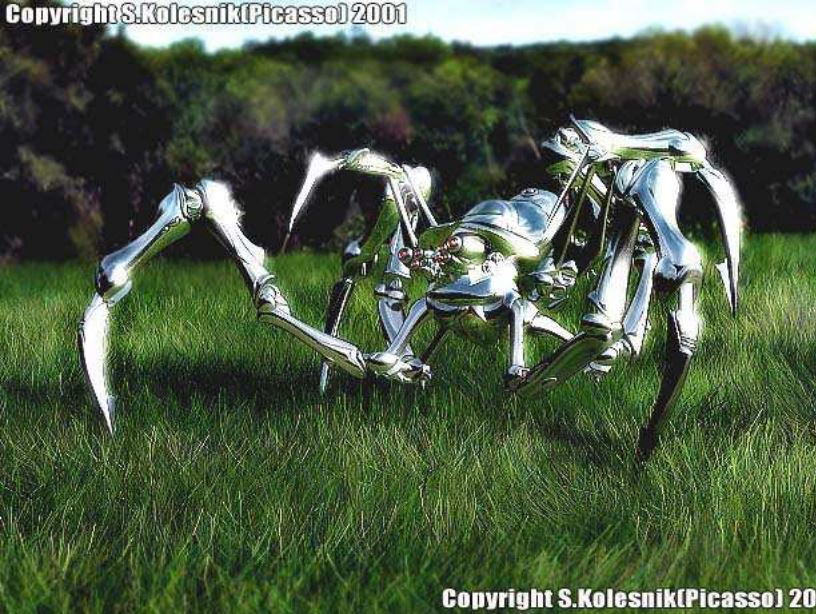
\includegraphics[width=0.75\textwidth]{Cap2/spiderrobot}
\caption{Cupim cibernético.}\label{FDIII}
\end{figure}

Considerando um robô manipulador rígido, malha aberta, e de $n$-juntas em série. Seja $q$ a representação de seu vetor de posição angular das juntas  e $\tau$ a representação de seu vetor de torque. A equação dinâmica pelo método de
Lagrange é dada por:
\begin{equation} \label{eq:lagr1}
\frac{d}{dt}(\frac{\partial L}{\partial \dot{q}})-\frac{\partial L}{\partial q}=\tau^{T}.
\end{equation}
O Lagrangiano $L$ é definido como a diferença entre as energias cinética e potencial do sistema:
\begin{equation} \label{L}
L=T-P
\end{equation}

A energia cinética total dos ligamentos é representada:
\begin{equation} \label{energT}
T=\frac{1}{2}\dot{q}^{T}M(q)\dot{q}
\end{equation}
